\documentclass[11pt,letterpaper,titlepage]{article}

%================== Document nomenclature
\newcommand{\DOCSUBJT}{Whitepaper: }   %Put document subject here
\newcommand{\DOCTITLE}{                      %Put document title here
	Incompressible Navier-Stokes equations using Finite Volume spatial discretization
}       
\newcommand{\DOCDATE} {April, 2020}         %Put document date here
\newcommand{\DOCREV}  {Rev 0.00}             %Put revision number here

%================== Misc Settings
\usepackage{fancyhdr}
\usepackage[left=0.75in, right=0.75in, bottom=1.0in]{geometry}
\usepackage{lastpage}
\usepackage{titleref}
\usepackage{booktabs}
\usepackage{appendix}

\appendixtitleon
\appendixtitletocon

\makeatletter

%================== List of figures and tables mods
\usepackage{tocloft}
\usepackage[labelfont=bf]{caption}

\renewcommand{\cftfigpresnum}{Figure\ }
\renewcommand{\cfttabpresnum}{Table\ }

\newlength{\mylenf}
\settowidth{\mylenf}{\cftfigpresnum}
\setlength{\cftfignumwidth}{\dimexpr\mylenf+3.5em}
\setlength{\cfttabnumwidth}{\dimexpr\mylenf+1.5em}



%=================== Graphics
\usepackage{graphicx}
\usepackage[breakwords]{truncate}
\usepackage{float}
\usepackage{array}
\usepackage{amsmath}
\usepackage{mdframed}
\usepackage{fancyvrb}
\usepackage{float}
\usepackage{cancel}
\usepackage{amssymb}
\graphicspath{ {images/} }
\usepackage[usenames,dvipsnames,svgnames,table]{xcolor}
%\usepackage[defaultlines=2,all]{nowidow}
\usepackage{listings}
\usepackage{color}
\definecolor{Brown}{cmyk}{0,0.81,1,0.60}
\definecolor{OliveGreen}{cmyk}{0.64,0,0.95,0.40}
\definecolor{CadetBlue}{cmyk}{0.62,0.57,0.23,0}
\usepackage{pdflscape}
\usepackage{relsize}
\usepackage{verbatim}
\usepackage{tabto}
%\usepackage{upgreek}
\usepackage{enumitem}
%\usepackage{MnSymbol}% http://ctan.org/pkg/mnsymbol
\usepackage[pdf]{graphviz}
\usepackage[linesnumbered,lined,boxruled,algosection,commentsnumbered]{algorithm2e}
\usepackage{enumitem}
\usepackage{bm} %Bold math
\usepackage{bbold} %mathbb{1}

\definecolor{gray}{rgb}{0.4,0.4,0.4}
\definecolor{darkblue}{rgb}{0.0,0.0,0.6}
\definecolor{cyan}{rgb}{0.0,0.6,0.6}

\definecolor{ao(english)}{rgb}{0.0, 0.5, 0.0}

\newcommand{\xmltag}[1]{\textcolor{blue}{ \texttt{#1}} }
\newcommand{\xmloption}[1]{\textcolor{ao(english)}{ \texttt{#1}} }


\counterwithin{figure}{section}
\renewcommand{\thefigure}{\arabic{section}.\arabic{figure}}
%=================== Big cdot
\newcommand*\bigcdot{\mathpalette\bigcdot@{.5}}
\newcommand*\bigcdot@[2]{\mathbin{\vcenter{\hbox{\scalebox{#2}{$\m@th#1\bullet$}}}}}


\newcommand{\beq}{\begin{equation*}
\begin{aligned}}
\newcommand{\eeq}{\end{aligned}
\end{equation*}}

\newcommand{\beqn}{\begin{equation}
	\begin{aligned}}
\newcommand{\eeqn}{\end{aligned}
	\end{equation}}

\newcommand{\bnabla}{\boldsymbol{\nabla}}
\newcommand{\bvel}{\mathbf{u}}
\newcommand{\pluseq}{\mathrel{+}=}
\newcommand{\asteq}{\mathrel{*}=}
	

%=================== Settings
\renewcommand{\baselinestretch}{1.2}
\definecolor{gray}{rgb}{0.4 0.4 0.4}
\newcommand{\stimes}{{\times}}

%================== Code syntax highlighting
\lstset{language=C++,frame=ltrb,framesep=2pt,basicstyle=\linespread{0.8} \small,
	keywordstyle=\ttfamily\color{OliveGreen},
	identifierstyle=\ttfamily\color{CadetBlue}\bfseries,
	commentstyle=\color{Brown},
	stringstyle=\ttfamily,
	showstringspaces=true,
	tabsize=2,}
	
%================== Section numbers with equation numbers
\numberwithin{equation}{section}


%================== Short \to arrow
\setlength{\medmuskip}{0mu}
%\newcommand{\tos}[1][3pt]{\mathrel{%
%   \hbox{\rule[\dimexpr\fontdimen22\textfont2-.2pt\relax]{#1}{.4pt}}%
%   \mkern-4mu\hbox{\usefont{U}{lasy}{m}{n}\symbol{41}}}}



\setlength\parindent{0pt}


\begin{document}

\begin{titlepage}
	\pagestyle{fancy}
	\vspace*{1.0cm}
	\centering
	\vspace{1cm}
	\vspace{.25cm}
	{\Large\bfseries  \DOCSUBJT \par} 
	{\Large\bfseries \DOCTITLE  \par}
	\vspace{1cm}
	{\Large \DOCDATE \par}
	\vspace{1.0cm}
	{\Large Jan Vermaak \par}
	{\Large \DOCREV \par}
	\begin{center}
			\begin{minipage}[c]{0.45\textwidth}
				\begin{figure}[H]
					
					
\includegraphics[width=3in]{Logo2_Medium.png}
				\end{figure}
			\end{minipage}
		\end{center}

\end{titlepage}	


\pagestyle{fancy}
\rfoot{Page \thepage \ of \pageref{LastPage}}
\cfoot{}
\lfoot{\truncate{14cm}{\DOCTITLE}}
\rhead{}
\chead{\currentname}
\lhead{}
\renewcommand{\footrulewidth}{0.4pt}

\newpage
\chead{Table of contents}
%\begin{comment}
\tableofcontents
\addtocontents{toc}{~\hfill\textbf{Page}\par}

\listoffigures
\listoftables

%\end{comment}
\chead{Contents}	

%#########################################################################
\newpage
\chead{The incompressible Navier-Stokes equations}
\section{The incompressible Navier-Stokes equations}
Conservation of mass (continuity equation):
\beqn
\frac{\partial \rho}{\partial t} +
\bnabla \bigcdot (\rho \bvel) = 0
\eeqn 

where $\rho$ is the fluid density, $\bvel$ is the fluid velocity vector with components $\bvel = [u_x, u_y, u_z]$.
\newline 
\newline
Conversion of momentum:
\beqn
\frac{\partial(\rho \bvel)}{dt} 
+ \bnabla \bigcdot ( \rho \bvel \otimes \bvel )
=  \mathbf{f} -\bnabla p
+ \bnabla \bigcdot \boldsymbol{\tau} 
\eeqn
\newline
where $\mathbf{f}$ is a body force vector (gravity,magnetism,etc.), $p$ is scalar static pressure, $ \boldsymbol{\tau} $ is the viscous shear-stress forces defined as

\beq
 \boldsymbol{\tau} 
= \bnabla \bigcdot \{ \mu \bnabla \bvel \} 
+ \bnabla \bigcdot \{ \mu (\bnabla \bvel)^T \}
- \frac{2}{3} \bnabla ( \mu \bnabla \bigcdot \bvel ).
\eeq 
\newline
The components of $ \boldsymbol{\tau} $ can also be denoted with indices along $i,j=1,2,3$. The entries of a combined tensor representation is defined by

\beq 
\tau_{ij} &= \mu \biggr [
\frac{\partial u_i}{\partial x_j} + \frac{\partial u_j}{\partial x_i} 
- \frac{2}{3}\delta_{ij}\frac{\partial u_k}{\partial x_k}
\biggr]
\quad \quad \quad &k=1,2,3
\eeq 
\newline
with $x_0=x$, $x_1=y$ and $x_2=z$. This tensor defines the shear-stress forces along the six cartesian planes as

\beq
\tau_{xx} &= 
\frac{2}{3} \mu \biggr ( 2\frac{\partial u_x}{\partial x} - \frac{\partial u_y}{\partial y} - \frac{\partial u_z}{\partial z} \biggr) \\
\tau_{yy} &= 
\frac{2}{3} \mu \biggr ( -\frac{\partial u_x}{\partial x} +2\frac{\partial u_y}{\partial y} - \frac{\partial u_z}{\partial z} \biggr) \\
\tau_{zz} &= 
\frac{2}{3} \mu \biggr ( -\frac{\partial u_x}{\partial x} - \frac{\partial u_y}{\partial y} +2 \frac{\partial u_z}{\partial z} \biggr) \\
\tau_{xy} &= \tau_{yx} = \mu \biggr( \frac{\partial u_y}{\partial x} + \frac{\partial u_x}{\partial y} \biggr) \\
\tau_{xz} &= \tau_{zx} = \mu \biggr( \frac{\partial u_z}{\partial x} + \frac{\partial u_x}{\partial z} \biggr) \\
\tau_{yz} &= \tau_{zy} = \mu \biggr( \frac{\partial u_z}{\partial y} + \frac{\partial u_y}{\partial z} \biggr)
\eeq 

or more compactly

\beq
\tau = 
\begin{bmatrix}
\tau_{xx} & \tau_{xy} & \tau_{xz} \\
\tau_{yx} & \tau_{yy} & \tau_{yz} \\
\tau_{zx} & \tau_{zy} & \tau_{zz} \\
\end{bmatrix}
\eeq 





\newpage 
\section{Some necessary tools}

\subsection{Tensors}
\subsubsection{Tensor product of two vectors, $\mathbf{a}\otimes \mathbf{b}$}
Also called the dyadic product. In many textbooks the general notation $\{\bvel \bvel\}$ or $\{ \bnabla \bvel \}$ is adopted which might not be intuitive to scholars unfamiliar with tensors. In this notation the $\{\}$ indicates that the terms within forms a tensor. The more technically correct representation would be the \textbf{tensor product notation} where we take the tensor product of two vectors, i.e., $\mathbf{a}$ and $\mathbf{b}$, both of the same dimension $N$, resulting in tensor of order $2$, as

\beqn 
\{\mathbf{a} \mathbf{b} \} = 
\mathbf{a} \otimes \mathbf{b} 
=
\begin{bmatrix}
a_0 \\ a_1 \\ \vdots \\ a_{N-1}
\end{bmatrix}
\otimes 
\begin{bmatrix}
b_0 \\ b_1 \\ \vdots \\ b_{N-1}
\end{bmatrix}
=
\begin{bmatrix}
a_0 b_0 & a_0 b_1 & \hdots & a_0 b_{N-1} \\
a_1 b_0 & a_1 b_1 & \hdots & a_1 b_{N-1} \\
\vdots   & \vdots   & \ddots & \vdots \\
a_{N-1} b_0 & a_{N-1} b_1 & \hdots & a_{N-1} b_{N-1} \\
\end{bmatrix}.
\eeqn 
\newline 
Note here that the ``order" of the tensor is also sometimes referred to as the tensor's rank. A simple definition of ``rank" is the number of indices in a given dimension required to address the components of a tensor. Therefore the above tensor has dimension $N$ and rank $2$. A scalar has dimension $1$ rank $0$ because we do not need any index, and a vector has dimension $N$ and rank $1$ because we only need a single index. In fluid mechanics we mostly deal with tensors of rank $2$.

\subsubsection{Vector inverse, $\mathbf{a}^{-1}$}
There is not a common notation for taking the component-wise inverse of a vector, however, the notation $\mathbf{a}^{-1}$ will be used to denote

\beqn
\mathbf{a}^{-1} = 
\begin{bmatrix}
\frac{1}{a_0} \\
\frac{1}{a_1} \\
\vdots  \\
\frac{1}{a_{N-1}}
\end{bmatrix}
\eeqn 

\subsubsection{Component-wise multiplication of vectors, $\mathbf{a}\mathbf{b}$}
Also called the Hadamard-product which is the component-wise multiplication of two vectors or two matrices, where both operands need to be the same size. The notation for a Hadamard-product is the symbol $\circ$ or $\odot$. The tensor product notation is also sometimes confusingly mixed with component-wise multiplication (i.e., $\mathbf{a}\mathbf{b}$ vs $\{ \mathbf{a}\mathbf{b} \}$ ), however the component-wise multiplication is
\beqn
\mathbf{a}\mathbf{b} = 
\mathbf{a} \circ \mathbf{b} = 
\mathbf{a} \odot \mathbf{b} = 
\begin{bmatrix}
a_0 b_0 \\
a_1 b_1 \\
\vdots \\
a_{N-1}b_{N-1}
\end{bmatrix}
\eeqn

\subsubsection{Component-wise division of vectors, $\mathbf{a}^{-1}\mathbf{b}$}
Also called Hadamard division where again both operands need to be of the same size. This is another instance of component-wise operations and involves the use of a vector-inverse, $\mathbf{a}^{-1}\mathbf{b}$, or simply written as division, $\mathbf{b}/\mathbf{a}$, in which case
\beqn
\mathbf{a}^{-1}\mathbf{b} =
\mathbf{b}/\mathbf{a} =  
\mathbf{b} \oslash \mathbf{a} =
\begin{bmatrix}
b_0/a_0  \\
b_1/a_1 \\
\vdots \\
b_{N-1}/a_{N-1}
\end{bmatrix}.
\eeqn
Again notice the absence of the tensor notation, $\{\}$.

\subsubsection{Commutativity of component-wise operations}
The following commutativity rules apply to component-wise operations:

\beqn
\alpha (\mathbf{a}\mathbf{b})&= (\alpha \mathbf{a}) \mathbf{b} = \mathbf{a}(\alpha \mathbf{b}) \\
\alpha (\mathbf{a}^{-1}\mathbf{b})&= (\alpha \mathbf{a}^{-1}) \mathbf{b} = \mathbf{a}^{-1}(\alpha \mathbf{b}) 
\\
\mathbf{c} \bigcdot (\mathbf{a}\mathbf{b})&= (\mathbf{c} \bigcdot \mathbf{a}) \mathbf{b} = \mathbf{a}(\mathbf{c} \bigcdot \mathbf{b}) \\
\mathbf{c} \bigcdot (\mathbf{a}^{-1}\mathbf{b})&= (\mathbf{c} \bigcdot \mathbf{a}^{-1}) \mathbf{b} = \mathbf{a}^{-1}(\mathbf{c} \bigcdot \mathbf{b}) 
\\
\alpha \mathbf{c} \bigcdot (\mathbf{a}\mathbf{b})&= (\alpha \mathbf{c} \bigcdot \mathbf{a}) \mathbf{b} = \mathbf{a}(\mathbf{c} \bigcdot \alpha \mathbf{b}) = \mathbf{c} \bigcdot (\alpha \mathbf{a} \mathbf{b} ) 
\eeqn 
where $\alpha$ is any scalar.

\subsubsection{Dot-product of a vector with a tensor, $\mathbf{a} \bullet \{t\}$}
Under the same topic of tensor product notation we can also discuss the \textbf{dot product of scalar and a rank 2 tensor}. The dot-product of a vector $\mathbf{a}$ and a tensor $\{ \mathbf{t}\}$, commonly written as $\mathbf{a} \bigcdot \{ \mathbf{t}\}$, which results in a vector of size $N$, can be understood using one of two thought patterns:

\begin{itemize}
\item Thought pattern 1: Classical component-wise dot product
\beqn 
\mathbf{a} \bigcdot \{ \mathbf{t}\} &=
\begin{bmatrix}
a_0 \\ a_1 \\ \vdots \\ a_{N-1}
\end{bmatrix}
\bigcdot 
\begin{bmatrix}
t_{00} & t_{01} & \hdots & t_{0(N-1)} \\
t_{10} & t_{11} & \hdots & t_{1(N-1)} \\
\vdots & \vdots & \ddots & \vdots \\
t_{(N-1)0} & t_{(N-1)1} & \hdots & t_{(N-1)(N-1)} \\
\end{bmatrix}\\
&=
\begin{bmatrix}
a_0 t_{00} &+ &a_1 t_{01} &+ &\hdots &+ &a_{N-1} t_{0(N-1)} \\
a_0 t_{10} &+ &a_1 t_{11} &+ &\hdots &+ &a_{N-1} t_{1(N-1)} \\
\vdots &+ &\vdots &+ &\ddots &+ &\vdots \\
a_0 t_{(N-1)0} &+ &a_1 t_{(N-1)1} &+ &\hdots &+ &a_{N-1} t_{(N-1)(N-1)} \\
\end{bmatrix}
\eeqn 

\item Thought pattern 2 (preferred): Dot product of vectors
\beqn 
\mathbf{a} \bigcdot \{ \mathbf{t}\} &=
\begin{bmatrix}
a_0 \\ a_1 \\ \vdots \\ a_{N-1}
\end{bmatrix}
\bigcdot 
\begin{bmatrix}
\mathbf{t}_0 \\
\mathbf{t}_1 \\
\vdots  \\
\mathbf{t}_{(N-1)}
\end{bmatrix}
=
\begin{bmatrix}
\mathbf{a} \ \bigcdot \ \mathbf{t}_0 \\
\mathbf{a} \ \bigcdot \ \mathbf{t}_1 \\
\vdots  \\
\mathbf{a} \ \bigcdot \ \mathbf{t}_{(N-1)}
\end{bmatrix}
\eeqn 
\end{itemize}
where the latter thought pattern requires the rank 2 tensor two be represented as a vector of vectors (or a matrix if you prefer).


\subsubsection{Dot-product of a vector with a tensor product of two other vectors, $\mathbf{a} \bullet \{\mathbf{b}\otimes \mathbf{c}\}$}
A special case relating to the dot product of a vector and a tensor is the notation $\mathbf{a} \ \bigcdot \ \{\mathbf{b} \otimes \mathbf{c} \}$, which commonly arises from an area vector's dot product with the velocity tensor (i.e. $\mathbf{A} \ \bigcdot \ \{ \bvel \otimes \bvel\}$). In such a case the non-linearity of $\bvel \otimes \bvel$ is removed by lagging the velocity as $\mathbf{A} \ \bigcdot  \ \{ \bvel^{(n)} \bvel^{(n-1)} \}$ for which we get the general form, $\mathbf{a} = \mathbf{A}$, $\mathbf{b} = \bvel^{(n)}$, $\mathbf{c} = \bvel^{(n-1)}$, such that

\beqn
\mathbf{a} \ \bigcdot \ \{\mathbf{b} \otimes \mathbf{c} \} &=
\mathbf{a} \ \bigcdot \ 
\begin{bmatrix}
b_0 c_0       & b_0 c_1       & \hdots & b_0 c_{N-1} \\
b_1 c_0       & b_1 c_1       & \hdots & b_1 c_{N-1} \\
\vdots         & \vdots        & \ddots & \vdots \\
b_{N-1} c_0 & b_{N-1} c_1 & \hdots & b_{N-1} c_{N-1} \\
\end{bmatrix} \\
&=
\begin{bmatrix}
a_0 b_0 c_0       & a_1 b_0 c_1       & \hdots & a_{N-1} b_0 c_{N-1} \\
a_0 b_1 c_0       & a_1 b_1 c_1       & \hdots & a_{N-1}  b_1 c_{N-1} \\
\vdots         & \vdots        & \ddots & \vdots \\
a_0 b_{N-1} c_0 & a_1 b_{N-1} c_1 & \hdots & a_{N-1}  b_{N-1} c_{N-1} \\
\end{bmatrix} \\
&=(\mathbf{a} \ \bigcdot \ \mathbf{c} ) \ \mathbf{b}
\eeqn 
\newline 
The usefulness of this will be made clearer in later sections.

\subsubsection{Divergence of a vector given its gradient, $\bnabla \bullet \mathbf{a} = \mathbb{1} \ \bullet \ \text{diag}(\bnabla \mathbf{a})$}
Programatically the divergence of vector-quantity can easily be obtained by accessing the diagonal elements of the gradient tensor, $\bnabla \mathbf{a}_{00}$, $\bnabla \mathbf{a}_{11}$ and $\bnabla \mathbf{a}_{22}$. Mathematically it can be written as

\beqn 
\bnabla \bullet \mathbf{a} = \mathbb{1} \ \bullet \ \text{diag}(\bnabla \mathbf{a})
\eeqn 

\vspace{1cm}
\subsection{Unstructured meshes and the treatment of certain quantities}
This section is meant to clarify some items found in a useful paper by Sezai \cite{Sezai} which deals with unstructured meshes and the finite volume method. Figure \ref{fig:faceaverages} below contains a graphic depiction of unstructured 2D cells which we will use to define numerous concepts.

\begin{figure}[H]
\centering
\includegraphics[width=0.5\linewidth]{Figures/FaceAverages}
\caption{Reference vector layout for neighboring cells}
\label{fig:faceaverages}
\end{figure}

The points $\mathbf{P}$, $\mathbf{N}$ and $\mathbf{F}$ are the present-cell-, neighboring-cell- and adjoining-face-centroids, respectively. The vector $\mathbf{PN}$ is from $\mathbf{P}$ to $\mathbf{N}$, and the projection of $\mathbf{PF}$ onto $\mathbf{PN}$ is at point $\mathbf{F}_i$. The vector $\mathbf{e}_{PN}$ is the unit vector along $\mathbf{PN}$ computed from $\mathbf{PN}/d_{PN}$, where $d_{PN} = || \mathbf{PN} ||_2$. The vector $\mathbf{e}_t$ is the unit tangential vector formed from $\mathbf{e}_t = \mathbf{e}_{PN} - \mathbf{n}$, with $\mathbf{n}$ being the face normal. The distance from $\mathbf{P}$ to $\mathbf{F}_i$, $d_{PF_i}$, is computed as 
$
d_{PF_i} = \mathbf{PF} \ \bigcdot  \ \mathbf{e}_{PN}
$, 
and $\mathbf{F}_i = \mathbf{P} + d_{PF_i}  \ \mathbf{e}_{PN}$.


\subsubsection{Linear interpolation of a quantity $\phi$ to a face, option 1}
A linear interpolation of any quantity $\phi$, to find $\phi_{f_i}$, can be determined by defining $r_P = \frac{d_{PF_i}}{d_{PN}}$ from which 
\beqn \label{eq:linear_interpolation_nocorr}
\phi_{f_i} &= (1-r_P) \phi_P + (r_P)\phi_N.
\eeqn
This is however not the desired value at the cell centroid, i.e. $\phi_f$. To correct for this we can linearly interpolate the gradient of $\phi$ to $\mathbf{F}_i$ and extend towards $\mathbf{F}$ as
\beq 
\bnabla \phi_{f_i} = (1-r_P) \bnabla \phi_P + (r_P)\bnabla \phi_N
\eeq 
using the vector from $\mathbf{F}_i$ to $\mathbf{F}$, $\mathbf{F_iF}$, to get
\beqn \label{eq:linear_interpolation}
\phi_f \approx \phi_{f_i}
+ \bnabla \phi_{f_i} \bigcdot \mathbf{F_iF}
\eeqn
which can be used for the interpolation of the pressure and/or temperature. Note however, that this form is not suitable for the interpolation of the velocity, which requires special treatment.

\subsubsection{Linear interpolation of a quantity $\phi$ to a face, option 2}
For quantities that are not very sensitive to variation in the direction of the face skewness, i.e., fluid viscosity, $\mu$, fluid density, $\rho$, and thermal conductivity, $k$, one can apply a less accurate, but still suitable interpolation, by neglecting the gradients and using the normal distance to the face. This requires $r_f$ defined as
\beqn 
r_f = \frac{
\mathbf{PF} \bigcdot \mathbf{n}
}{
\mathbf{PF} \bigcdot \mathbf{n} +
\mathbf{FN} \bigcdot \mathbf{n}
}
\eeqn 

which can then be used to linearly interpolated quantities as
\beqn \label{eq:linear_interpolation_nocorr2}
\phi_{f_i} &= (1-r_f) \phi_P + (r_f)\phi_N.
\eeqn

\subsubsection{Computing gradients}
There are different methods for computing gradients of the form $\bnabla \phi$. 
\newline
\newline
\textbf{Green-Gauss:}\newline
This formulation is identical to ``Option 3" of chapter 9.2 in the book by Moukalled et al. \cite{MMD}.
The first order Green-Gauss approximation reduces essentially to a summation over faces.

\beqn \label{eq:gradient_gg} 
\bnabla \phi = \frac{1}{V} \sum_f \mathbf{A}_f \phi_f
\eeqn 

where $\phi_f$ is taken as a linear interpolation between the adjoining face's cells. This formulation poses some challenges when undetermined faces fluxes are encountered, as is the case with boundaries and unstructured meshes, and therefore we require an algorithm to compensate. Therefore the following algorithm is applied:

\begin{enumerate}
\item Assume $\bnabla \phi^{(n-1)} = 0$
\item Compute $\bnabla \phi^{(n)}$ over the entire domain using $\frac{1}{V}\sum_f \mathbf{A}_f \phi_f$ where $\phi_f$ is computed from \eqref{eq:linear_interpolation} as
\beq
\phi_f &= 
(1-r_P) \phi_P + (r_P)\phi_N + 
\biggr [
(1-r_P) \bnabla \phi_P + (r_P)\bnabla \phi_N
\biggr ]^{(n-1)} \bigcdot \mathbf{F_iF}
\eeq 
and boundary faces are computed as
\beq 
\phi_b = \phi_P + \bnabla \phi_P^{(n-1)} \bigcdot  \ \mathbf{PF}
\eeq 

\item Compute $|| \bnabla \phi^{(n)} - \bnabla \phi^{(n-1)} ||_2$. If $|| \bnabla \phi^{(n)} - \bnabla \phi^{(n-1)} ||_2<\epsilon$ then terminate.

\item Swap $\bnabla \phi^{(n)}$ and $\bnabla \phi^{(n-1)}$.
\item Repeat 2 to 4.
\end{enumerate}

\textbf{Least squares:}\newline
TBC  

\subsubsection{Flux of a gradient}
A diffusion quantity that often arises in unstructured meshes is $\mathbf{A}_f \bigcdot (\bnabla \phi)_f$, where $\mathbf{A}_f$ is the area vector formed by the face area $A_f$ and its normal $n$ as $\mathbf{A}_f = A_f \mathbf{n}$. When we deal with skewed faces, this diffusion  term needs some treatment. In general, since the face is skewed, the flux at the cell face develops additional components other than the orthogonal component along the direction of $\mathbf{PN}$.  These additional components are not intuitive to understand and the paper by Sezai \cite{Sezai} lacks explanation of some of the items in its graphical illustrations. Refer to Figure \ref{fig:faceaveragesskewed} for the following discussion.

\begin{figure}[H]
\centering
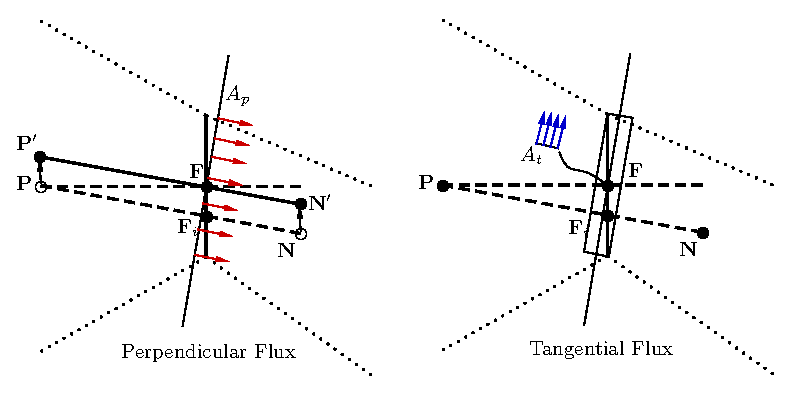
\includegraphics[width=0.8\linewidth]{Figures/FaceAveragesSkewed}
\caption{Decomposed areas for the interpolation of a gradient flux}
\label{fig:faceaveragesskewed}
\end{figure}

Given that the correct way to approximate the flux across the face is to compute the gradient along its centroid, we require the gradient to be computed from $\phi_{P'}$ and $\phi_{N'}$ along the projected perpendicular area $A_p$. Additionally we need to compute the flux along the tangential area $A_t$. Including these terms within an implicit formulation is, however, cumbersome to say the least. Instead we include explicit corrections.
\newline
\newline
Firstly, we formulate the fluxes at $\mathbf{P}'$ and $\mathbf{N}'$ (see the left schematic in Figure \ref{fig:faceaveragesskewed}) as 

\beq 
\phi_{P'} &= \phi_P + (\bnabla \phi)_P^{(n-1)} \  \bigcdot  \ \mathbf{F_iF} \\
\phi_{N'} &= \phi_N + (\bnabla \phi)_N^{(n-1)} \  \bigcdot \  \mathbf{F_iF}
\eeq 
\newline
where $\mathbf{F_iF}$ is the vector from $\mathbf{F}_i$ to $\mathbf{F}$ and the gradients are computed from the previous iteration's flux field. The perpendicular gradient term can then be computed from

\beq 
\biggr (
\mathbf{A}_f \bigcdot (\bnabla \phi)_f 
\biggr)_p
&=
\frac{A_p}{d_{PN}} \biggr ( \phi_{N'} - \phi_{P'} \biggr)
\\
&= \frac{A_p}{d_{PN}} \biggr ( \phi_{N} - \phi_{P} \biggr)
+  \frac{ A_p }{d_{PN}} \biggr ( (\bnabla \phi)_N  -  (\bnabla \phi)_P \biggr)^{(n-1)}
\ \bigcdot \mathbf{F_iF} 
\eeq 
\newline 
where $A_p = A_f / (\mathbf{e}_{PN} \bigcdot \mathbf{n})$. Secondly, the tangential component can be computed from \eqref{eq:linear_interpolation}.

\beq 
\biggr (
\mathbf{A}_f \bigcdot (\bnabla \phi)_f 
\biggr)_t
&= (\bnabla \phi)_F \bigcdot \mathbf{A}_t
\\
&\approx  (\bnabla \phi)_{F_i}^{(n-1)} \bigcdot \mathbf{A}_t
\eeq 
\newline
where $\mathbf{A}_t = \mathbf{A}_f - A_p \mathbf{e}_{PN}$ and the gradient at the face centroid is approximated by the gradient interpolated at $\mathbf{F}_i$ which is not an unreasonable approximation considering that cell skewness is normally minimized. 
Putting it all together we have

\beqn \label{eq:flux_of_gradient}
\mathbf{A}_f \bigcdot (\bnabla \phi)_f 
=
 \frac{A_p}{d_{PN}} \biggr ( \phi_{N} - \phi_{P} \biggr)
+  \frac{ A_p }{d_{PN}} \biggr ( (\bnabla \phi)_N  -  (\bnabla \phi)_P \biggr)^{(n-1)}
\ \bigcdot \mathbf{F_iF} 
+
 (\bnabla \phi)_{F_i}^{(n-1)} \bigcdot \mathbf{A}_t
\eeqn 
\newline
This equation appears in the momentum equation as well as the pressure correction equation for the SIMPLE method.









\newpage 
\section{Discretization of the momentum equation}
We start our derivations with the conservation of momentum equation where the non-linear convective term, 
$\bnabla\bigcdot ( \rho \bvel \otimes \bvel ) $, has been linearized through the use of the velocity at a previous iteration $(n-1)$, and the time derivative has been taken as linearly changing from timestep $(t-1)$,


\beq
\rho \frac{\bvel - \bvel^{(t-1)}}{\Delta t} 
+ \bnabla \bigcdot ( \rho \bvel^{(n-1)} \otimes \bvel )
\ - \ \bnabla \bigcdot \{ \mu \bnabla \bvel \} 
&= -\bnabla p + \bnabla \bigcdot  \{ \mu (\bnabla \bvel)^T \}
\ - \ \frac{2}{3}\bnabla \cdot (\mu \bnabla \bigcdot \bvel^{(n-1)})
+ \mathbf{f}.
\eeq
\newline
Next we integrate this equation over a given cell's volume and apply Gauss' divergence theorem. We then also convert surface integrals to sum over areas of the faces. In the latter process we combine the area of a face, $A_f$, with its associated normal, $\mathbf{n}_f$, and introduce the area vector, $\mathbf{A}_f = A_f \mathbf{n}_f$,

\beq 
\frac{\rho_P V_P}{\Delta t} (\bvel - \bvel^{(t-1)})
&+ \int_S \mathbf{n} \bigcdot ( \rho \bvel \otimes \bvel^{(n-1)} ).dA
\ - \ \int_S \mathbf{n} \bigcdot \{ \mu \bnabla \bvel \}.dA \\
&= -V_P (\bnabla p)^{(n-1)}
+ \int_S \mathbf{n} \bigcdot  \{ \mu (\bnabla \bvel)^T \}^{(n-1)}.dA 
\ - \ \frac{2}{3}\int_S \mathbf{n} \cdot (\mu \bnabla \bigcdot \bvel^{(n-1)}).dA
+ V_P \mathbf{f}
\eeq 
and after application of Green's theorem,
\beqn 
\therefore
\frac{\rho_P V_P}{\Delta t} \bvel 
&+ \sum_f   \dot{m}_f^{(n-1)}  \bvel_f
\ - \ \sum_f \mathbf{A}_f \bigcdot \{ \mu \bnabla \bvel \}_f \\
&=-V_P (\bnabla p)^{(n-1)}
+ \sum_f \mathbf{A}_f \bigcdot  \{ \mu (\bnabla \bvel)^T \}_f^{(n-1)} 
\ - \ \frac{2}{3}\sum_f \mathbf{A}_f \cdot (\mu \bnabla \bigcdot \bvel^{(n-1)})_f
+\frac{\rho_P V_P}{\Delta t} \bvel^{(t-1)}
+ V_P \mathbf{f}.
\eeqn
\newline 
Note here that we used the property $\mathbf{a} \bigcdot ( \mathbf{b} \otimes \mathbf{c}) = (\mathbf{a} \bigcdot \mathbf{c} )\mathbf{b}$, defined in the tools section, to get
\beq
\int_S \mathbf{n} \bigcdot ( \rho \bvel \otimes \bvel^{(n-1)} ).dA 
&= 
\int_S \biggr ( \mathbf{n} \bigcdot (\rho\bvel^{(n-1)}) \biggr )  \bvel.dA \\
&=
\sum_f \biggr ( \rho_f \mathbf{A}_f \bigcdot \bvel_f^{(n-1)} \biggr ) \bvel_f \\
&=
\sum_f \dot{m}_f^{(n-1)} \bvel_f \\
\eeq 

\subsection{Preface on the need for $\bnabla \bvel$}
The gradient of the velocity cannot simply be computed, i.e., from the Green-Gauss method in \eqref{eq:gradient_gg}, because we are using a collocated scheme for which it is known to create a phenomenon known as ``checkerboarding". This is especially true since we require the face-velocities. Checkerboarding was first addressed in a paper by Rhie and Chow \cite{RhieChow} by applying momentum interpolation and was later improved on by Majumdar \cite{Majumdar}. In this project we use the Majumdar Momentum Interpolation Method (MMIM) \textbf{which we will detail later}.
\newline
\newline 
\textcolor{red}{Note:} For now, assume that we can compute $\bnabla \bvel$ and have its previous iteration value, $\bnabla \bvel^{(n-1)}$, available.
\newline
\newline
We now require expressions for the face terms $\dot{m}_f^{(n-1)} \bvel_f$, $\{ \mu \nabla \bvel\}_f$, $\{ \mu (\nabla \bvel)^T\}_f$, and $(\mu \bnabla \bigcdot \bvel^{(n-1)})_f$. In all the sub-sections that follow we will be working with a known mass flow rate $\dot{m}_f = \rho \mathbf{A}_f \bigcdot \bvel_f^{(\ell-1)} $ which will be assumed zero at the start of the simulation but will be updated and stored later.
\newline
\newline
But first let us define the coefficient formulation.

\subsection{Coefficient formulation and under-relaxation}

When applying the discretization of the momentum equation above, we ultimately seek to arrange algebraic terms into the following general form:
\beq 
\mathbf{a}^P \bvel^P + \sum_f \mathbf{a}^N \bvel^N = \mathbf{b}_{nur}^P + \sum_f -\mathbf{A}_f p_f
\eeq 
\beq
\therefore
\mathbf{a}^P \bvel^P  = - \sum_f \mathbf{a}^N \bvel^N + \mathbf{b}_{nur}^P + \sum_f -\mathbf{A}_f p_f
\eeq
where the coefficients $\mathbf{a}^P$ and $\mathbf{a}^N$ are vector valued and $\mathbf{b}_{nur}$ signifies no under-relaxation. 
For iterative control we further introduce an under-relaxation with respect to the previous iteration velocity such that 

\beq 
\mathbf{a}^P \bvel^P  = 
\alpha_u \biggr (
- \sum_f \mathbf{a}^N \bvel^N + \mathbf{b}_{nur}^P + \sum_f -\mathbf{A}_f p_f
\biggr) 
+
(1-\alpha_u) a^P (\bvel^P)^{(n-1)}
\eeq 

\beq
\therefore
\frac{1}{\alpha_u} \mathbf{a}^P \bvel^P  = 
- \sum_f \mathbf{a}_f^N \bvel^N +
\mathbf{b}_{nur}^P \ + \ \frac{1-\alpha_u}{\alpha_u} \ \mathbf{a}^P (\bvel^P)^{(n-1)}
+ \sum_f -\mathbf{A}_f p_f
\eeq

Finally we combine the previous iteration under-relaxed velocity with $\mathbf{b}_{nur}$ as $\mathbf{b} = \mathbf{b}_{nur} + \ + \ \frac{1-\alpha_u}{\alpha_u} \ \mathbf{a} (\bvel)^{(n-1)}$
to get the \textbf{momentum equation in coefficient form}:

\beqn \label{eq:momentum_coefficient_form}
\therefore
\frac{1}{\alpha_u} \mathbf{a}^P \bvel^P  = 
- \sum_f \mathbf{a}_f^N \bvel^N +
\mathbf{b}^P 
+ \sum_f -\mathbf{A}_f p_f
\eeqn
Note here that the $\mathbf{a}$ and $\mathbf{b}$ coefficients are vector valued.


\subsection{Material properties at faces, $\mu_f$ and $\rho_f$}
Material properties are generally not as rapidly varying as the pressure or velocity and therefore we linearly interpolate these values without the correction term specified in \eqref{eq:linear_interpolation} and instead just use \eqref{eq:linear_interpolation_nocorr2}. Therefore,
\beqn
\mu_f = (1-r_f)\mu_P + (r_f)\mu_N 
\eeqn
\beqn
\rho_f = (1-r_f)\rho_P + (r_f)\rho_N 
\eeqn

\subsection{Diffusion gradient terms, $\{ \mu \nabla \bvel \}_f$}
The gradient-term, $\mathbf{A}_f \bigcdot \{ \mu \bnabla \bvel \}_f$ is treated as introduced in \eqref{eq:flux_of_gradient},

\beqn
-\mathbf{A}_f \bigcdot ( \mu\bnabla \bvel)_f 
&=
 -\mu_f \frac{A_p}{d_{PN}} \biggr ( \bvel_N - \bvel_P \biggr)
-  \mu_f \frac{ A_p }{d_{PN}} \biggr \{ \bnabla \bvel_N  -  \bnabla \bvel_P \biggr\}^{(n-1)}
\ \bigcdot \mathbf{F_iF} \\
&\quad-\mu_f
\biggr \{
(1-r_P)\bnabla \bvel_P+(r_P)\bnabla \bvel_N
\biggr \}^{(n-1)} \bigcdot \mathbf{A}_t
\eeqn 
\newline
Note here that this formulation has both implicit terms and explicit terms. The coefficients get updated as 
\beq 
\mathbf{a}^N &= \mathbf{a}^N -  \ \mu_f \frac{A_p}{d_{PN}} \cdot \mathbb{1} \\
\mathbf{a}^P &= \mathbf{a}^P + \  \mu_f \frac{A_p}{d_{PN}} \cdot \mathbb{1} \\
\mathbf{b}^P &= \mathbf{b}^P + \   
\mu_f \frac{ A_p }{d_{PN}} \biggr \{ \bnabla \bvel_N  -  \bnabla \bvel_P \biggr\}^{(n-1)}
\ \bigcdot \mathbf{F_iF} \ + \ \mu_f
\biggr \{
(1-r_P)\bnabla \bvel_P+(r_P)\bnabla \bvel_N
\biggr \}^{(n-1)} \bigcdot \mathbf{A}_t
\eeq 

\subsection{Cross-diffusion gradient terms, $\{ \mu (\nabla \bvel)^T \}_f^{(n-1)}$}
This term can be evaluated purely using explicitly values and by noting the term has a weak coupling to the momentum equation, we can apply the interpolation option given in \eqref{eq:linear_interpolation_nocorr2}

\beqn 
\mathbf{A}_f \bigcdot \{ \mu (\nabla \bvel)^T \}_f^{(n-1)} = 
\mu_f \mathbf{A}_f \bigcdot
\biggr \{
(1-r_f)
\{\nabla \bvel\}_P^T
+
(r_f)
\{\nabla \bvel\}_N^T
\biggr\}^{(n-1)}
\eeqn 

The coefficients get updated as 
\beq
\mathbf{b}^P &= \mathbf{b}^P 
+ \ 
\mu_f \mathbf{A}_f \bigcdot
\biggr \{
(1-r_f)
\{\nabla \bvel\}_P^T
+
(r_f)
\{\nabla \bvel\}_N^T
\biggr\}^{(n-1)}
\eeq



\subsection{Divergence term, $(\mu \bnabla \bullet \mathbf{u}^{(n-1)})_f$}

The divergence term is easy to obtain if we already computed the gradients at the faces. For this we use the notation defined in the tools section.

\beqn 
-\frac{2}{3}\mathbf{A}_f (\mu \bnabla \bigcdot \bvel^{(n-1)})_f =
-\frac{2}{3} \mu_f \mathbf{A}_f 
\biggr(
\mathbb{1} \  \bigcdot \ 
 \text{diag}(\bnabla \bvel) 
\biggr)_f^{(n-1)}
\eeqn 

The coefficients get updated as 
\beq
\mathbf{b}^P &= \mathbf{b}^P 
- \ \frac{2}{3} \mu_f \mathbf{A}_f 
\biggr(
\mathbb{1} \  \bigcdot \ 
 \text{diag}(\bnabla \bvel) 
\biggr)_f^{(n-1)}
\eeq

\subsection{Face convection term, $\dot{m}_f^{(n-1)} \bvel_f $ }

The face convective term is taken from a second-order upwind scheme. This is achieved by considering the upstream face velocity as $\bvel_f^U$ as pertaining to the associated upstream cell (either the present cell or the neighbor cell) as captured by

\beqn 
\dot{m}_f^{(n-1)} \bvel_f^U &= 
\text{min}\biggr ( 
\dot{m}_f^{(n-1)},0.0
\biggr ) \bvel^N +
\text{max}\biggr ( 
\dot{m}_f^{(n-1)},0.0
\biggr ) \bvel^P \\
&\quad + \ \dot{m}_f^{(n-1)}
\begin{cases}
\bnabla \bvel_N^{(n-1)} \bigcdot \mathbf{NF}, \quad \quad \quad &\text{if } \dot{m}_f^{(n-1)}<0 \\
\bnabla \bvel_P^{(n-1)} \bigcdot \mathbf{PF}, \quad \quad \quad &\text{if } \dot{m}_f^{(n-1)}>0 \\
\end{cases}
\eeqn 
\newline
where again $\mathbf{PF}$ is the vector from the present cell centroid to the face centroid, and $\mathbf{NF}$ is the vector from the neighboring cell centroid to the face centroid. The neighbor $N$ is the neighbor at face $f$.
\newline
\newline
The coefficients get updated as 
\beq 
\mathbf{a}^N &= \mathbf{a}^N + \ 
\text{min}\biggr ( 
\dot{m}_f^{(n-1)},0.0
\biggr )\\
\mathbf{a}^P &= \mathbf{a}^P + \ 
\text{max}\biggr ( 
\dot{m}_f^{(n-1)},0.0
\biggr )\\
\mathbf{b}^P &= \mathbf{b}^P - \   
\dot{m}_f^{(n-1)}
\begin{cases}
\bnabla \bvel_N^{(n-1)} \bigcdot \mathbf{NF}, \quad \quad \quad &\text{if } \dot{m}_f^{(n-1)}<0 \\
\bnabla \bvel_P^{(n-1)} \bigcdot \mathbf{PF}, \quad \quad \quad &\text{if } \dot{m}_f^{(n-1)}>0 \\
\end{cases}
\eeq 




\subsection{Face pressure, $p_f$}

The face pressure is simply taken as a geometrically averaging of the adjoining cell's pressures when the face is internal, as depicted in \eqref{eq:linear_interpolation}, and is interpolated to the boundary when the face is on a boundary. Therefore, with an internal face we have
\beq 
p_{f_i} = ( 1-r_P) p_P  + (r_P)p_N
\eeq 
\beq 
\bnabla p_{f_i}^{(n-1)} = ( 1-r_P) \bnabla p_P^{(n-1)}  + (r_P) \bnabla p_N^{(n-1)}
\eeq 
and then
\beqn
p_f = p_{f_i} + \bnabla p_{f_i}^{(n-1)} \bigcdot \mathbf{F_iF}
\eeqn 
and for a boundary face we have 
\beq 
p_f = p_P + \bnabla p_P^{(n-1)} \bigcdot \mathbf{PF}.
\eeq 
\newline
Note again here that we need to store the gradient of the pressure.




\newpage
\section{Segregated solver (The SIMPLE method)}
The momentum equation can be segregated from its implicit connection with the pressure by using the previous iteration's pressure field to solve an intermediate velocity, $\bvel_0$, and using explicit values for the pressure

\beqn
\frac{1}{\alpha_u} \mathbf{a}^P \bvel_0^P  = 
- \sum_f \mathbf{a}_f^N \bvel_0^N +
\mathbf{b}^P 
+ \sum_f -\mathbf{A}_f p_f^{(n-1)}
\eeqn
\newline
The formulation of a pressure correction follows from the fact that the velocity, computed from a guessed pressure field, does not satisfy the continuity equation, that is

\beq 
\frac{\partial \rho}{\partial t} + 
\bnabla \bigcdot (\rho \bvel_0) &\approx
\frac{\rho^P - (\rho^P)^{(t-1)}}{\Delta t} + 
\frac{1}{V_P}\sum_f \rho \mathbf{A}_f \bigcdot \bvel_0 \ne 0 \\
\therefore 
\frac{\rho^P - (\rho^P)^{(t-1)}}{\Delta t}V_P + \sum_f \dot{m}_{f0} &\ne 0
\eeq 
\newline
We then postulate a mass flux correction, $\dot{m}_{f}'$, such that

\beqn \label{eq:pcorr1}
 \frac{\rho^P - (\rho^P)^{(t-1)}}{\Delta t}V_P + 
\sum_f \biggr (
\dot{m}_{f0} +
 \dot{m}_{f}'  
\biggr ) &= 0
\eeqn

and then apply a strategy to obtain a relation to pressure. Suppose we use the newly computed velocity field, $\bvel_0$, to isolate and compute a pressure gradient on a face. We could do this by reapplying \eqref{eq:momentum_coefficient_form}, but instead of treating the pressure gradient as a known we make this the unknown. For the present cell $P$  this takes the form

\beqn \label{eq:pcorr2}
\frac{1}{\alpha_u} \mathbf{a}^P \bvel_0^P  = 
- \sum_f \mathbf{a}_f^N \bvel_0^N +
\mathbf{b}^P 
-V_P (\bnabla p)^P
\eeqn

for which we can arrange the pressure gradient to the left hand side

\beqn \label{eq:pcorr3}
-V_P (\bnabla p)^P = \frac{1}{\alpha_u} \mathbf{a}^P \bvel_0^P + \sum_f \mathbf{a}_f^N \bvel_0^N -\mathbf{b}^P
\eeqn
From this we see that we can make a correction to the velocity of the form

\beq 
-V_P (\bnabla p')_P &= \frac{1}{\alpha_u}\mathbf{a}_P \  \bvel_P ' 
\\
\therefore
\bvel_P' &=- \alpha_u V_P \mathbf{a}_P^{-1} (\bnabla p')_P
\eeq 
\newline
When we then plug this expression into \eqref{eq:pcorr1} we get a Laplacian-like equation

\beq 
\rho \bnabla \bigcdot \bvel_0 + \rho \bnabla \bigcdot \bvel' &= 0 \\
\rho \bnabla \bigcdot \bvel_0 + \rho \bnabla \bigcdot  (-\alpha_u V \mathbf{a}^{-1} \bnabla p') &= 0 
\\
\therefore
-\bnabla \bigcdot  (\rho \alpha_u V \mathbf{a}^{-1} \bnabla p') &=
-\rho \bnabla \bigcdot \bvel_0
\eeq

Discretizing this equation leads to
\beq 
\sum_f - \mathbf{A}_f \bigcdot  (\rho \alpha_u V_f \mathbf{a}_f^{-1} \bnabla p_f')
&= \sum_f -\rho \mathbf{A}_f \bigcdot \bvel_{0f}.
\eeq 
Note here the appearance of $\mathbf{A}_f \bigcdot \bnabla p_f'$ which technically needs to be treated as described in \eqref{eq:flux_of_gradient}, however, since no explicit information for $\bnabla p'$ is available from previous iterations, we cannot make the skewness corrections. Fortunately, since $p'$ tends to zero upon convergence, we can neglect these corrections.

\beq 
\sum_f - \mathbf{A}_f \bigcdot  (\rho \alpha_u V_f \mathbf{a}_f^{-1} \bnabla p_f')
&= \sum_f -\rho \mathbf{A}_f \bigcdot \bvel_{0f}
\\
\sum_f - \rho \alpha_u V_f
\mathbf{A}_f \bigcdot   \mathbf{a}_f^{-1} \mathbf{s}_\Delta^{-1}(p^N - p^P)')
&= \sum_f -\dot{m}_{0f}
\eeq 
which can be solved using a diffusion-type solver. After the solution is obtained we can correct certain quantities by noting
\beq 
\dot{m}_f' &= \rho \mathbf{A}_f \bigcdot \bvel_f' = -\rho \alpha_u V_f \mathbf{A}_f \bigcdot \mathbf{a}_f^{-1} \bnabla p_f'
\eeq 
and then applying the following:
\beq 
\dot{m}_f &= \dot{m}_{0f} + \dot{m}_f'
\\
\bvel &= \bvel_0 - \alpha_u V_P \mathbf{a}_P^{-1} (\bnabla p')_P 
\\
p &= p^{(n-1)} + \alpha_p p'
\eeq 


\subsection{Computing face velocities}
When using a collocated grid scheme the process of computing the face velocities, $\bvel_f$, which is required to determine $\dot{m}_f$ and $\bnabla u$, cannot simply be accomplished by applying the linear interpolation depicted in \eqref{eq:linear_interpolation} because it results in the well known phenomenon of pressure``checkerboarding". A solution to this problem is to use the Majumdar Momemtum Interpolation Method (MIM) which is a modification of the Rhie-Chow MIM, and can be derived as follows:
\newline
\newline
We start with the momentum equation at the adjoining cells of a face in the same form as what we used to derive the pressure correction equation, recall \eqref{eq:pcorr2}, but now we write the equations for both the present cell, $P$, and the neighboring cell, $N$:

\beq
\frac{1}{\alpha_u} \mathbf{a}^P \bvel^P  = 
- \sum_f \mathbf{a}_f^N \bvel^N +
\mathbf{b}^P 
-V_P (\bnabla p)^P
\eeq

\beq
\frac{1}{\alpha_u} \mathbf{a}^N \bvel^N  = 
- \sum_f \mathbf{a}_f^N \bvel^N +
\mathbf{b}^N
-V_N (\bnabla p)^N
\eeq

We can define the following to simplify these equations:

\beqn
\mathbf{H}^P &= -\sum_f \mathbf{a}_f^N \bvel^N \quad \quad \quad \text{w.r.t.}  \ P \\
\mathbf{H}^N &= -\sum_f \mathbf{a}_f^N \bvel^N \quad \quad \quad \text{w.r.t.}  \ N 
\eeqn

with the simplified equations now

\beq
\frac{1}{\alpha_u} \mathbf{a}^P \bvel^P  = 
\mathbf{H}^P +
\mathbf{b}^P
-V_P (\bnabla p)^P
\eeq

\beq
\frac{1}{\alpha_u} \mathbf{a}^N \bvel^N  = 
\mathbf{H}^N +
\mathbf{b}^N
-V_N (\bnabla p)^N
\eeq
\newline
With yet another simplification we define $\bvel_{mim} = \mathbf{H} + \mathbf{b}$ as a \textbf{pseudo-velocity} that can be computed and stored for each cell. Our reduced equations are now

\beq
\frac{1}{\alpha_u} \mathbf{a}^P \bvel^P  = \bvel_{mim}^P - V_P (\bnabla p)^P
\eeq

\beq
\frac{1}{\alpha_u} \mathbf{a}^N \bvel^N  = \bvel_{mim}^N - V_N (\bnabla p)^N
\eeq

We then interpolate all the coefficient and terms but leave the interpolated $\bvel$ and $\bnabla p$ to get

\beqn
\frac{1}{\alpha_u} \biggr(
(1-r_P)\mathbf{a}^P + (r_P)\mathbf{a}^N
\biggr ) \bvel_f  
= \biggr(
(1-r_P)\bvel_{mim}^P + (r_P)\bvel_{mim}^N
\biggr )
-\biggr(
(1-r_P)V_P + (r_P)V_N
\biggr ) (\bnabla p)_f
\eeqn 

or more generally
\beqn
\frac{1}{\alpha_u} \mathbf{a}_f \bvel_f  
= \bvel_{mim}^f
-V_f (\bnabla p)_f
\eeqn 

after which we get the \textbf{Momentum Interpolated velocity} as

\beqn \label{eq:MIM_velocity}
 \bvel_f  
= \alpha_u \mathbf{a}_f^{-1} \biggr(
\bvel_{mim}^f
-V_f (\bnabla p)_f.
\biggr)
\eeqn 
\newline
In this equation $(\bnabla p)_f$ can then be computed using \eqref{eq:linear_interp_gradient}.



\newpage
\chead{References}
\begin{thebibliography}{1}
    
    \bibitem{Sezai} Sezai I., {\em Implementation of boundary conditions in pressure-based finite volume methods on unstructured grids}, Numerical Heat Transfer, Part B: Fundamentals, 2017
    
    \bibitem{MMD} Moukalled F., Mangani L., Darwish M., {\em The Finite Volume Method in Computational Fluid Dynamics - An Advanced Introduction with OpenFOAM and Matlab}, Springer, 2016.
    
    \bibitem{RhieChow} Rhie C.M., Chow W.L., {\em Numerical Study of the Turbulent Flow Past an Airfoil with Trailing Edge Separation}, AIAAJ Volume 21, Number 11, November 1983.
    
    \bibitem{Majumdar} Majumdar S., {\em Role of underrelaxation in momentum interpolation for calculation of flow with nonstaggered grids}, Numerical Heat Transfer 13, pages 125-132. 1998.
    
    
\end{thebibliography}





\end{document}